\begin{figure}[htbp]\centering
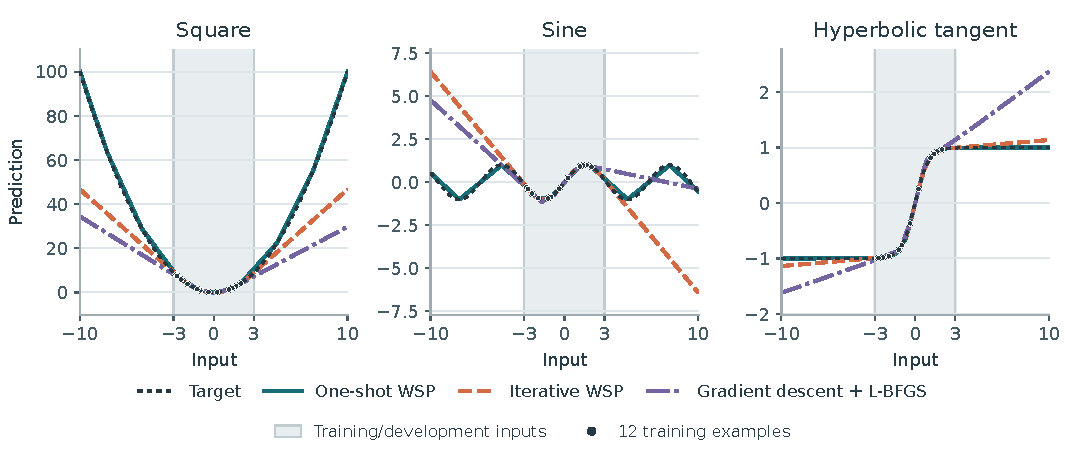
\includegraphics[width=\linewidth]{prediction_curves.pdf}
\caption{\textbf{Improved central fit can coexist with a worse extrapolation rule.} Each panel uses a 16-unit scalar network with 50 coefficients, the first recorded random start (164), and examples-only WSP. Shading marks the training and development interval; dots are the twelve training pairs. Curves are evaluations of the frozen networks, not averages over runs. These illustrative regressions show how similar central predictions conceal different outer continuations; they do not estimate how often this happens. Tables~\ref{tab:focusouter} and~\ref{tab:sizes_outer} summarize errors across all three starts.}\label{fig:prediction-curves}
\end{figure}
